\begin{frame}
    \centering
    \frametitle{Queues}
    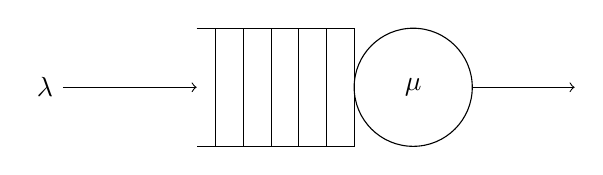
\begin{tikzpicture}
        \draw[->] (-0.7,-0.75) node[left] {\(\lambda\)} -- (1,-0.75);
        \draw (1,0) -- ++(2cm,0) -- ++(0,-1.5cm) -- ++(-2cm,0);
        \foreach \i in {1,...,5}
            \draw (3cm-\i*10pt,0) -- +(0,-1.5cm);
        \draw (3.75, -0.75) circle [radius=0.75cm];
        \node at (3.75, -0.75) {\(\mu\)};
        \draw[->] (4.5, -0.75) -- (5.8, -0.75);
    \end{tikzpicture}

    % \vspace{1cm}
    % \pause
    % \begin{tikzpicture}[-, node distance = 0.7cm]
    %     \node[state] (zero) {0};
    %     \node[state, right=of zero] (one) {1};
    %     \node[state, right=of one] (two) {2};
    %     \node[state, right=of two] (three) {3};
    %     \node[state, right=of three, draw=none] (infinity) {\( \dots \)};
    %     \draw[every loop]
    %         (zero) edge[bend left] node [above] {\( \lambda \)} (one)
    %         (one) edge[bend left] node [above] {\( \lambda \)} (two)
    %         (two) edge[bend left] node [above] {\( \lambda \)} (three)
    %         (three) edge[bend left] node [above] {\( \lambda \)} (infinity)
    %         (infinity) edge[bend left] node [below] {\( \mu \)} (three)
    %         (three) edge[bend left] node [below] {\( \mu \)} (two)
    %         (two) edge[bend left] node [below] {\( \mu \)} (one)
    %         (one) edge[bend left] node [below] {\( \mu \)} (zero)
    %     ;
    % \end{tikzpicture}
\end{frame}



\begin{frame}
    \frametitle{Queueing representation of hospital}
    \centering
    \begin{figure}[h]
        \centering
        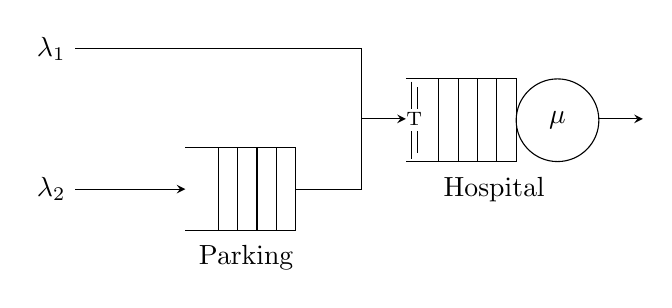
\begin{tikzpicture}[>=stealth, scale=0.7] %arrow type
            % Queue 1
            \draw (1,0) -- ++(2cm,0) -- ++(0,-1.5cm) -- ++(-2cm,0);
            \foreach \i in {1,...,4}
            \draw (3cm-\i*10pt,0) -- +(0,-1.5cm);

            % Queue 2
            \draw (5,1.25) -- ++(2cm,0) -- ++(0,-1.5cm) -- ++(-2cm,0);
            \foreach \i in {1,...,4}
            \draw (7cm-\i*10pt,1.25) -- +(0,-1.5cm);
            \draw (7.75,0.5) circle [radius=0.75cm];
            \node at (7.75, 0.5) {\(\mu\)};

            % The two vertical lines at the very start of Queue 2
            \draw (7cm-54pt,1.2) -- +(0,-0.5cm);
            \draw (7cm-54pt,0.3) -- +(0,-0.5cm);
            \draw (7cm-51pt,1.1) -- +(0,-0.4cm);
            \draw (7cm-51pt,0.3) -- +(0,-0.4cm);
            \node[anchor=north] at (5.15, 0.83 cm) {\scriptsize{T}};

            % the arrows and labels (Queue 1+2)
            \node[align=center] at (1cm,-2cm) {};
            \node[align=center] at (6cm,-0.75cm) {};

            % Arrows lines
            \draw (4.2, 1.8) -- +(-5.2,0) node[left] {\( \lambda_1 \)};
            \draw[<-] (1,-0.75) -- +(-2,0) node[left] {\( \lambda_2 \)};
            \draw[->] (4.2, 0.525) -- (5, 0.525);
            \draw[->] (8.5,0.525) -- (9.3,0.525);

            % Parking and Hospital Labels
            \node[align=center] at (2.1cm,-2cm) {Parking};
            \node[align=center] at (6.6cm,-0.75cm) {Hospital};

            % Others lines
            \draw[-] (3,-0.75) -- (4.2,-0.75);
            \draw (4.2, 0.525) -- (4.2, -0.75);
            \draw (4.2, 1.8) -- (4.2, 0.525);

        \end{tikzpicture}
    \end{figure}

    \small
    \begin{itemize}
        \item \( \lambda_1 \): Arrival rate of non-ambulance patients
        \item \( \lambda_2 \): Arrival rate of ambulance patients
        \item \( \mu \): Service rate
        \item \( T \): Threshold
    \end{itemize}
\end{frame}



% \begin{frame}
%     \frametitle{Queueing representation of hospital}
%     \centering

%     \begin{tikzpicture}[>=stealth, scale=0.6]
%         % Queue 1
%         \draw (1,0) -- ++(2cm,0) -- ++(0,-1.5cm) -- ++(-2cm,0);
%         \foreach \i in {1,...,4}
%         \draw (3cm-\i*10pt,0) -- +(0,-1.5cm);
%         \draw (1, 0) -- ++ (0, -1.5cm);
        
%         % Queue 2
%         \draw (5,1.25) -- ++(2cm,0) -- ++(0,-1.5cm) -- ++(-2cm,0);
%         \foreach \i in {1,...,4}
%         \draw (7cm-\i*10pt,1.25) -- +(0,-1.5cm);
%         \draw (7.65,1.8) circle [radius=0.62cm];
%         \draw (7.65,0.5) circle [radius=0.62cm];
%         \draw (7.65,-0.8) circle [radius=0.62cm];

%         % The two vertical lines at the very start of Queue 2 
%         \draw (7cm-54pt,1.2) -- +(0,-0.5cm);
%         \draw (7cm-54pt,0.3) -- +(0,-0.5cm);        
%         \draw (7cm-51pt,1.1) -- +(0,-0.4cm);
%         \draw (7cm-51pt,0.3) -- +(0,-0.4cm);
%         \node[anchor=north] at (5.15, 0.85 cm) {\tiny{2}};

%         % Arrows lines
%         \draw (4.2, 1.8) -- +(-5.2,0) node[left] {\( \lambda_1 \)};
%         \draw[<-] (1,-0.75) -- +(-2,0) node[left] {\( \lambda_2 \)};
%         \draw[->] (4.2, 0.525) -- (5, 0.525);
%         \draw[->] (8.5,0.525) -- (9.3,0.525);
        
%         % Others lines
%         \draw[-] (3,-0.75) -- (4.2,-0.75);
%         \draw (4.2, 0.525) -- (4.2, -0.75);
%         \draw (4.2, 1.8) -- (4.2, 0.525);

%         % Animations
%         \only<2,3,4,5,6,7,8,9,10>{ % Stickman queue 1 - top
%             \node[draw=none, red] at (7.65,1.8) {\Strichmaxerl[1]};
%         }
%         \only<3,4,5,6,7,8,10>{ % Stickman queue 1 - mid
%             \node[draw=none, blue] at (7.65,0.5) {\Strichmaxerl[1]};
%         }
%         \only<4,5,6,7,8,9>{ % Stickman queue 1 - bottom - red
%             \node[draw=none, red] at (7.65, -0.8) {\Strichmaxerl[1]};
%         }
%         \only<6,7>{ % Stickman queue 1 - first
%             \node[draw=none, red] at (6.82, 0.5) {\Strichmaxerl[1]};
%         }
%         \only<5,6,7,8,9,10>{ % Stickman queue 2 - first
%             \node[draw=none, blue] at (2.82,-0.75) {\Strichmaxerl[1]};
%         }
%         \only<7,8,9>{ % Stickman queue 2 - second
%             \node[draw=none, blue] at (2.47,-0.75) {\Strichmaxerl[1]};
%         }
%         \only<2,4,6>{ % arrival 1
%             \draw[red, very thick] (4.2, 1.8) -- +(-5.2,0) node[left] {\( \lambda_1 \)};
%             \draw[red, very thick] (4.2, 1.8) -- (4.2, 0.525);
%             \draw[->, red, very thick] (4.2, 0.525) -- (5, 0.525);
%         }
%         \only<3,5,7>{ % arrival 2
%             \draw[<-, blue, very thick] (1,-0.75) -- +(-2,0) node[left] {\( \lambda_2 \)};
%         }
%         \only<3,10>{ % queue 1 to queue 2
%             \draw[-, blue, very thick] (3,-0.75) -- (4.2, -0.75);
%             \draw[blue, very thick] (4.2, 0.525) -- (4.2, -0.75);
%             \draw[->, blue, very thick] (4.2, 0.525) -- (5, 0.525);
%         }
%         \only<8,10>{ % exit arrival 1
%             \draw[->, red, very thick] (8.5,0.525) -- (9.3,0.525);
%         }
%         \only<9>{ % exit arrival 2
%             \draw[->, blue, very thick] (8.5,0.525) -- (9.3,0.525);
%         }
%     \end{tikzpicture}

%     \begin{figure}
%         \begin{tikzpicture}[-, node distance = 0.7cm, auto, every node/.style={scale=0.5}]
%             \node[state] (one) {(0,0)};
%             \node[state, right=of one] (two) {(0,1)};
%             \node[state, right=of two] (three) {(0,2)};
%             \node[state, right=of three] (four) {(0,3)};
%             \node[state, right=of four] (five) {(0,4)};
%             \node[state, below=of three] (three_one) {(1,2)};
%             \node[state, below=of three_one] (three_two) {(2,2)};
%             \node[state, below=of four] (four_one) {(1,3)};
%             \node[state, below=of four_one] (four_two) {(2,3)};
%             \node[state, below=of five] (five_one) {(1,4)};
%             \node[state, below=of five_one] (five_two) {(2,4)};
%             \draw[every loop]
%                 (one) edge[bend left] node {\( \lambda_1 + \lambda_2 \)} (two)
%                 (two) edge[bend left] node {\( \mu \)} (one)
%                 (two) edge[bend left] node {\( \lambda_1 + \lambda_2 \)} (three)
%                 (three) edge[bend left] node {\( 2\mu \)} (two)
%                 (three) edge[bend left] node {\( \lambda_1 \)} (four)
%                 (four) edge[bend left] node {\( 3\mu \)} (three)
%                 (four) edge[bend left] node {\( \lambda_1 \)} (five)
%                 (five) edge[bend left] node {\( 3\mu \)} (four)
%                 (three) edge[bend left] node {\( \lambda_2 \)} (three_one)
%                 (three_one) edge[bend left] node {\( 2\mu \)} (three)
%                 (three_one) edge[bend left] node {\( \lambda_1 \)} (four_one)
%                 (four_one) edge[bend left] node {\( 3\mu \)} (three_one)
%                 (four_one) edge[bend left] node {\( \lambda_1 \)} (five_one)
%                 (five_one) edge[bend left] node {\( 3\mu \)} (four_one)
%                 (four) edge node {\( \lambda_2 \)} (four_one)
%                 (five) edge node {\( \lambda_2 \)} (five_one)
%                 (three_one) edge[bend left] node {\( \lambda_2 \)} (three_two)
%                 (three_two) edge[bend left] node {\( 2\mu \)} (three_one)
%                 (four_one) edge node {\( \lambda_2 \)} (four_two)
%                 (five_one) edge node {\( \lambda_2 \)} (five_two)
%                 (three_two) edge[bend left] node {\( \lambda_1 \)} (four_two)
%                 (four_two) edge[bend left] node {\( 3\mu \)} (three_two)
%                 (four_two) edge[bend left] node {\( \lambda_1 \)} (five_two)
%                 (five_two) edge[bend left] node {\( 3\mu \)} (four_two)
%                 ;

%             \only<1>{\node[state, ultra thick] (one) {(0,0)};}
%             \only<2>{
%                 \node[state, ultra thick, red, right=of one] (two) {(0,1)};
%                 \draw[every loop, red] (one) edge[bend left] node {\( \lambda_1 + \lambda_2 \)} (two);
%             }
%             \only<3>{
%                 \node[state, ultra thick, blue, right=of two] (three) {(0,2)};
%                 \draw[every loop, blue] (two) edge[bend left] node {\( \lambda_1 + \lambda_2 \)} (three);
%             }
%             \only<4>{
%                 \node[state, ultra thick, red, right=of three] (four) {(0,3)};
%                 \draw[every loop, red] (three) edge[bend left] node {\( \lambda_1 \)} (four);
%             }
%             \only<5>{
%                 \node[state, ultra thick, blue, below=of four] (four_one) {(1,3)};
%                 \draw[every loop, blue] (four) edge node {\( \lambda_2 \)} (four_one);
%             }
%             \only<6>{
%                 \node[state, ultra thick, red, below=of five] (five_one) {(1,4)};
%                 \draw[every loop, red] (four_one) edge[bend left] node {\( \lambda_1 \)} (five_one);
%             }
%             \only<7>{
%                 \node[state, ultra thick, blue, below=of five_one] (five_two) {(2,4)};            
%                 \draw[every loop, blue] (five_one) edge node {\( \lambda_2 \)} (five_two);
%             }
%             \only<8>{
%                 \node[state, ultra thick, red, below=of four_one] (four_two) {(2,3)};         
%                 \draw[every loop, red] (five_two) edge[bend left] node {\( 3\mu \)} (four_two);
%             }
%             \only<9>{
%                 \node[state, ultra thick, blue, below=of three_one] (three_two) {(2,2)};
%                 \draw[every loop, blue] (four_two) edge[bend left] node {\( 3\mu \)} (three_two);
%             }
%             \only<10>{
%                 \node[state, ultra thick, red, below=of three] (three_one) {(1,2)};
%                 \draw[every loop, red] (three_two) edge[bend left] node {\( 2\mu \)} (three_one);
%             }
%         \end{tikzpicture}
%     \end{figure}
% \end{frame}
